\chapter{Distribución T de Student}

Esta distribución surge de la necesidad de estimar la \textbf{media} de una población normalmente distribuida pequeña. \cite{wiki:1}

\section{Descripción}

Aparece de manera natural al realizar la prueba t de Student para la determinación de las diferencias entre dos medias muestrales y para la construcción del intervalo de confianza para la diferencia entre las medias de dos poblaciones cuando se desconoce la desviación típica de una población y ésta debe ser estimada a partir de los datos de una muestra.


\section{PDF}
\begin{center}
	$P(X=\textit{x}) = \frac{\Gamma((v + 1) / 2)} {\sqrt{v\pi} \Gamma (v/2)} (1 + x^2 / v)^{-(v+1)/2} $
\end{center}

\subsection{Parámetros}
Los parámetros que usamos en las funciones de esta distribución son:

\begin{center}
	\begin{tabular} {| l | l |}
		\hline
		v & Grados de libertad \textit{N} $\in 1, 2, 3, ...$\\ \hline
	\end{tabular}
\end{center}

\section{CDF}
La función de distribución acumualada es:

\begin{center}
$\frac{1}{2} + x\Gamma(\frac{v+1}{2}) \frac{H}{\sqrt{v\pi} \Gamma (v/2)}$
\end{center}

Donde \textit{H} es la función Hipergeométrica.

\section{Media y Varianza}
\subsection{Media}
La esperanza de una variable aleatoria X con distribución hipergeométrica es:
\begin{center}
	$0$
\end{center}

\subsection{Varianza}
siendo su varianza
\begin{center}
	$\frac{v}{v-2}$
\end{center}

\section{MGF}
\textit{No definida}

\section{Gráficas}

\begin{center}	
	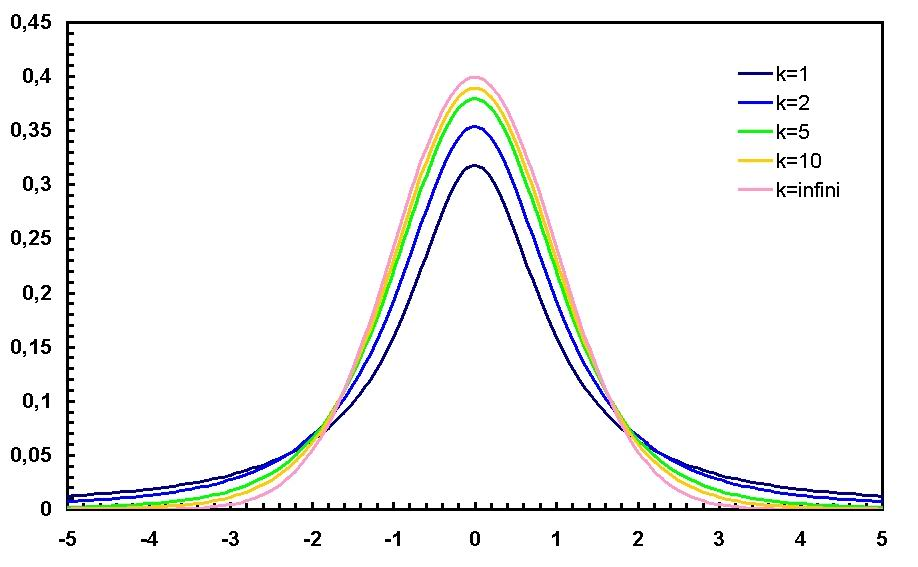
\includegraphics[scale=0.5]{imgs/t-pdf.jpeg}
	
	\textit{PDF}
\end{center}

\begin{center}	
	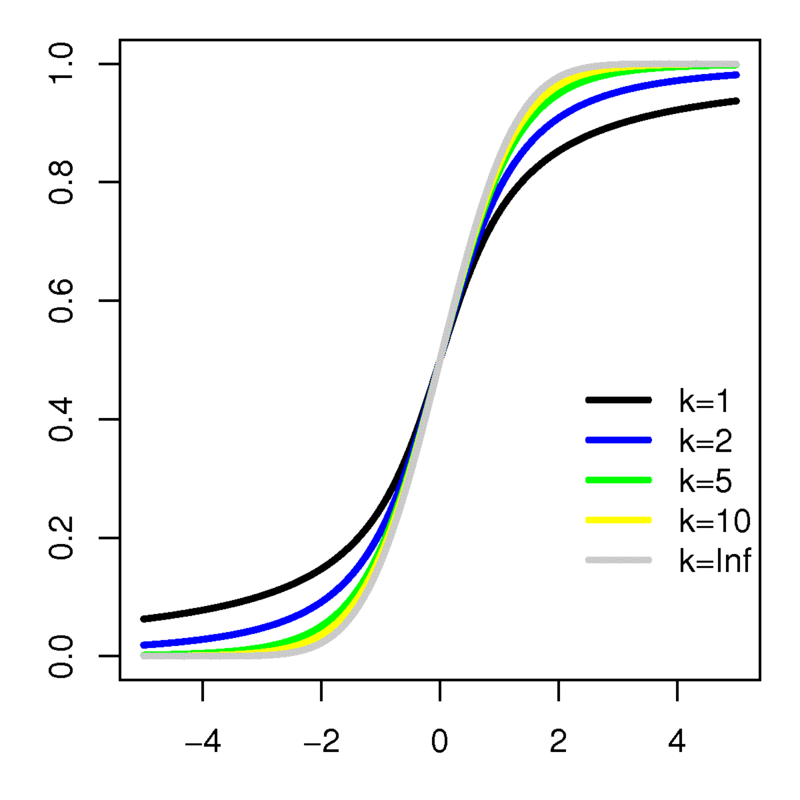
\includegraphics[scale=2]{imgs/t-cdf.png}
	
	\textit{CDF}
\end{center}


\section{Aplicaciones en la vida real}

Es aplicable cuando tenemos menos de 30 datos, y no conocemos la desviación estándar de la población y cuando la población de la extraemos la muestra está distribuida normalmente.